% This must be in the first 5 lines to tell arXiv to use pdfLaTeX, which is strongly recommended.
\pdfoutput=1
% In particular, the hyperref package requires pdfLaTeX in order to break URLs across lines.

\documentclass[11pt]{article}

% Remove the "review" option to generate the final version.
\usepackage{acl}

% Standard package includes
\usepackage{times}
\usepackage{latexsym}

% Custom package includes
\usepackage{easyReview}
\usepackage{booktabs}
\usepackage{array}
\usepackage{multirow}

% Custom commands
\newcommand\MyBox[1]{
  \fbox{\lower0.75cm
    \vbox to 1.7cm{\vfil
      \hbox to 1.7cm{\hfil\parbox{1.4cm}{#1}\hfil}
      \vfil}%
  }%
}

% For proper rendering and hyphenation of words containing Latin characters (including in bib files)
\usepackage[T1]{fontenc}
% For Vietnamese characters
% \usepackage[T5]{fontenc}
% See https://www.latex-project.org/help/documentation/encguide.pdf for other character sets

% This assumes your files are encoded as UTF8
\usepackage[utf8]{inputenc}

% This is not strictly necessary, and may be commented out,
% but it will improve the layout of the manuscript,
% and will typically save some space.
\usepackage{microtype}

\usepackage{graphicx}


% If the title and author information does not fit in the area allocated, uncomment the following
%
%\setlength\titlebox{<dim>}
%
% and set <dim> to something 5cm or larger.

\title{Perceptions and Sentiments Towards the Future of AI - Deep Learning on Internet Archive Data}

% Author information can be set in various styles:
% For several authors from the same institution:
% \author{Author 1 \and ... \and Author n \\
%         Address line \\ ... \\ Address line}
% if the names do not fit well on one line use
%         Author 1 \\ {\bf Author 2} \\ ... \\ {\bf Author n} \\
% For authors from different institutions:
% \author{Author 1 \\ Address line \\  ... \\ Address line
%         \And  ... \And
%         Author n \\ Address line \\ ... \\ Address line}
% To start a seperate ``row'' of authors use \AND, as in
% \author{Author 1 \\ Address line \\  ... \\ Address line
%         \AND
%         Author 2 \\ Address line \\ ... \\ Address line \And
%         Author 3 \\ Address line \\ ... \\ Address line}

\author{
    Dünya Baradari\\Leipzig University\And
    Finn Bartels\\Leipzig University\And
    Artur Dewald\\Leipzig University\And
    Julia Peters\\Leipzig University
}

\begin{document}
\maketitle
\begin{abstract}
For recent years digitization has been increasingly impacting our everyday lives.
More and more frequently new technologies are being introduced opening new possibilities.
Are these new AI systems offering previously unimagined opportunities or unprecedented threats?
Is humanity better off right now without further inventions originating from AI?
With our research we explore  the perceptions towards the future of AI.
Utilizing a web archive with data from the past ~10 years, we extract statements about AI. Subsequently we employ our Model Pipeline containing several models to identify phrases about the future and to assign an appropriate sentiment and a topic to them.
By analyzing these statements, we were able to determine a slightly positive tendency.
Moreover, our approach provides a possibility of analyzing statements for opinions about the future for any other subject than AI.

\end{abstract}

\graphicspath{
              {./figures/}
             }

\section{Introduction}

Human-like artificial intelligence (AI) has been exciting and frightening humanity since the antiquity.
Often intertwined with the concept of an artificial man, humanoid automata with the supposed capacity to answer questions and feel emotions have been present among all civilizations, including the ancient Egyptians and Greek \citep{Newquist1994}, Chinese \citep{cohen1986} and Mesopotamians \citep{unat2008}.
Yet, it has been in the past decades that the rise of computing power according to Moore’s Law has enabled a wide-scale application of AI technologies.
At the time of writing, use cases range from self-driving cars, personalization of ads in online browsing to highly complex predication tasks for protein folding \citep{jumper2021}.
\\
This rapid development of \emph{intelligent machines} in everyday life and application has led to both hopes and fears among the general population.
\citet{cave2019} identify four dichotomy categories of excitement and fears about artificial intelligence.
These are immortality and inhumanity, ease and obsolescence, gratification and alienation and dominance and uprising (Table~\ref{dichotomy-categories}).

%%%%%%%%%%%%%%%%%%%%%%%%%%%%%%%%%%%%%%%%%%%%%%%%%%%%%%%%%%%%%%%%%%%%%%%%%%%%%%%%%%%%%%%%%%%%%%%%%%%%%%%%%%%%%%%%%%%%%%%%%%%%%%%
%%%%%%%%%%%%%%%%%%%%%%%%%%%%%%%%%%%%%%%%%%%%%%%%%%%%%%%%%%%%%%%%%%%%%%%%%%%%%%%%%%%%%%%%%%%%%%%%%%%%%%%%%%%%%%%%%%%%%%%%%%%%%%%
\begin{table}[t]
    \centering
    \resizebox{\columnwidth}{!}{%
    \begin{tabular}{lll}
        \toprule
        \textbf{Dichotomy} & \textbf{Hope}  & \textbf{Fear} \\
        \midrule
        Immortality and Inhumanity & Much longer lives & Losing one's identity \\
        Ease and Obsolescence & Life free of work & Becoming redundant \\
        Gratification and Alienation & AI can fulfil one's desires & Humans will become redundant to each other \\
        Dominance and Uprising & AI offers power over others & AI will turn against humans \\
        \bottomrule
    \end{tabular}
    }
\caption{\label{dichotomy-categories}
Categories of dichotomies of hopes and fears towards AI.
Based on \citet{cave2019}.
They further argue that such perceptions, which may not align with reality, can yet influence the development, regulation, and applications of AI.
The encouragement of research into AI ethics by various public policy groups and governments may be a reflection of this point \citep{leslie2019}.
\\
Hence, it should be of great importance to policy makers, social scientists but also researchers working on artificial intelligence how general society perceives the future of the rapid advances in this field.
In our work, we employ a large language model approach to analyse Web Archive* data of the past ~10 years concerning statements about the future of AI.
Applying a topic clustering approach, we thereby seek to go beyond \citet{cave2019} categorisation and understand the most common topics regarding AI in online content.
By examining the prevalence and sentiment of clusters and topics within clusters, we can learn how to direct education, ethics, and research efforts for a better future with AI.
}
\end{table}
%%%%%%%%%%%%%%%%%%%%%%%%%%%%%%%%%%%%%%%%%%%%%%%%%%%%%%%%%%%%%%%%%%%%%%%%%%%%%%%%%%%%%%%%%%%%%%%%%%%%%%%%%%%%%%%%%%%%%%%%%%%%%%%
%%%%%%%%%%%%%%%%%%%%%%%%%%%%%%%%%%%%%%%%%%%%%%%%%%%%%%%%%%%%%%%%%%%%%%%%%%%%%%%%%%%%%%%%%%%%%%%%%%%%%%%%%%%%%%%%%%%%%%%%%%%%%%%

\section{Methodology}

For the realization of our concept, we aimed for the accomplishment of the following three objectives:

\begin{enumerate}
    \item Obtaining a sufficiently large dataset with different expressions about the topic of AI.
    \item Raw data transformation into a dataset that matches the target schema illustrated in \autoref{fig:overview}.
    \item Creation of a visualization from which society's perceptions on different topics of AI can be extracted.
\end{enumerate}%
%
%
\begin{figure}[t]
    \centering
    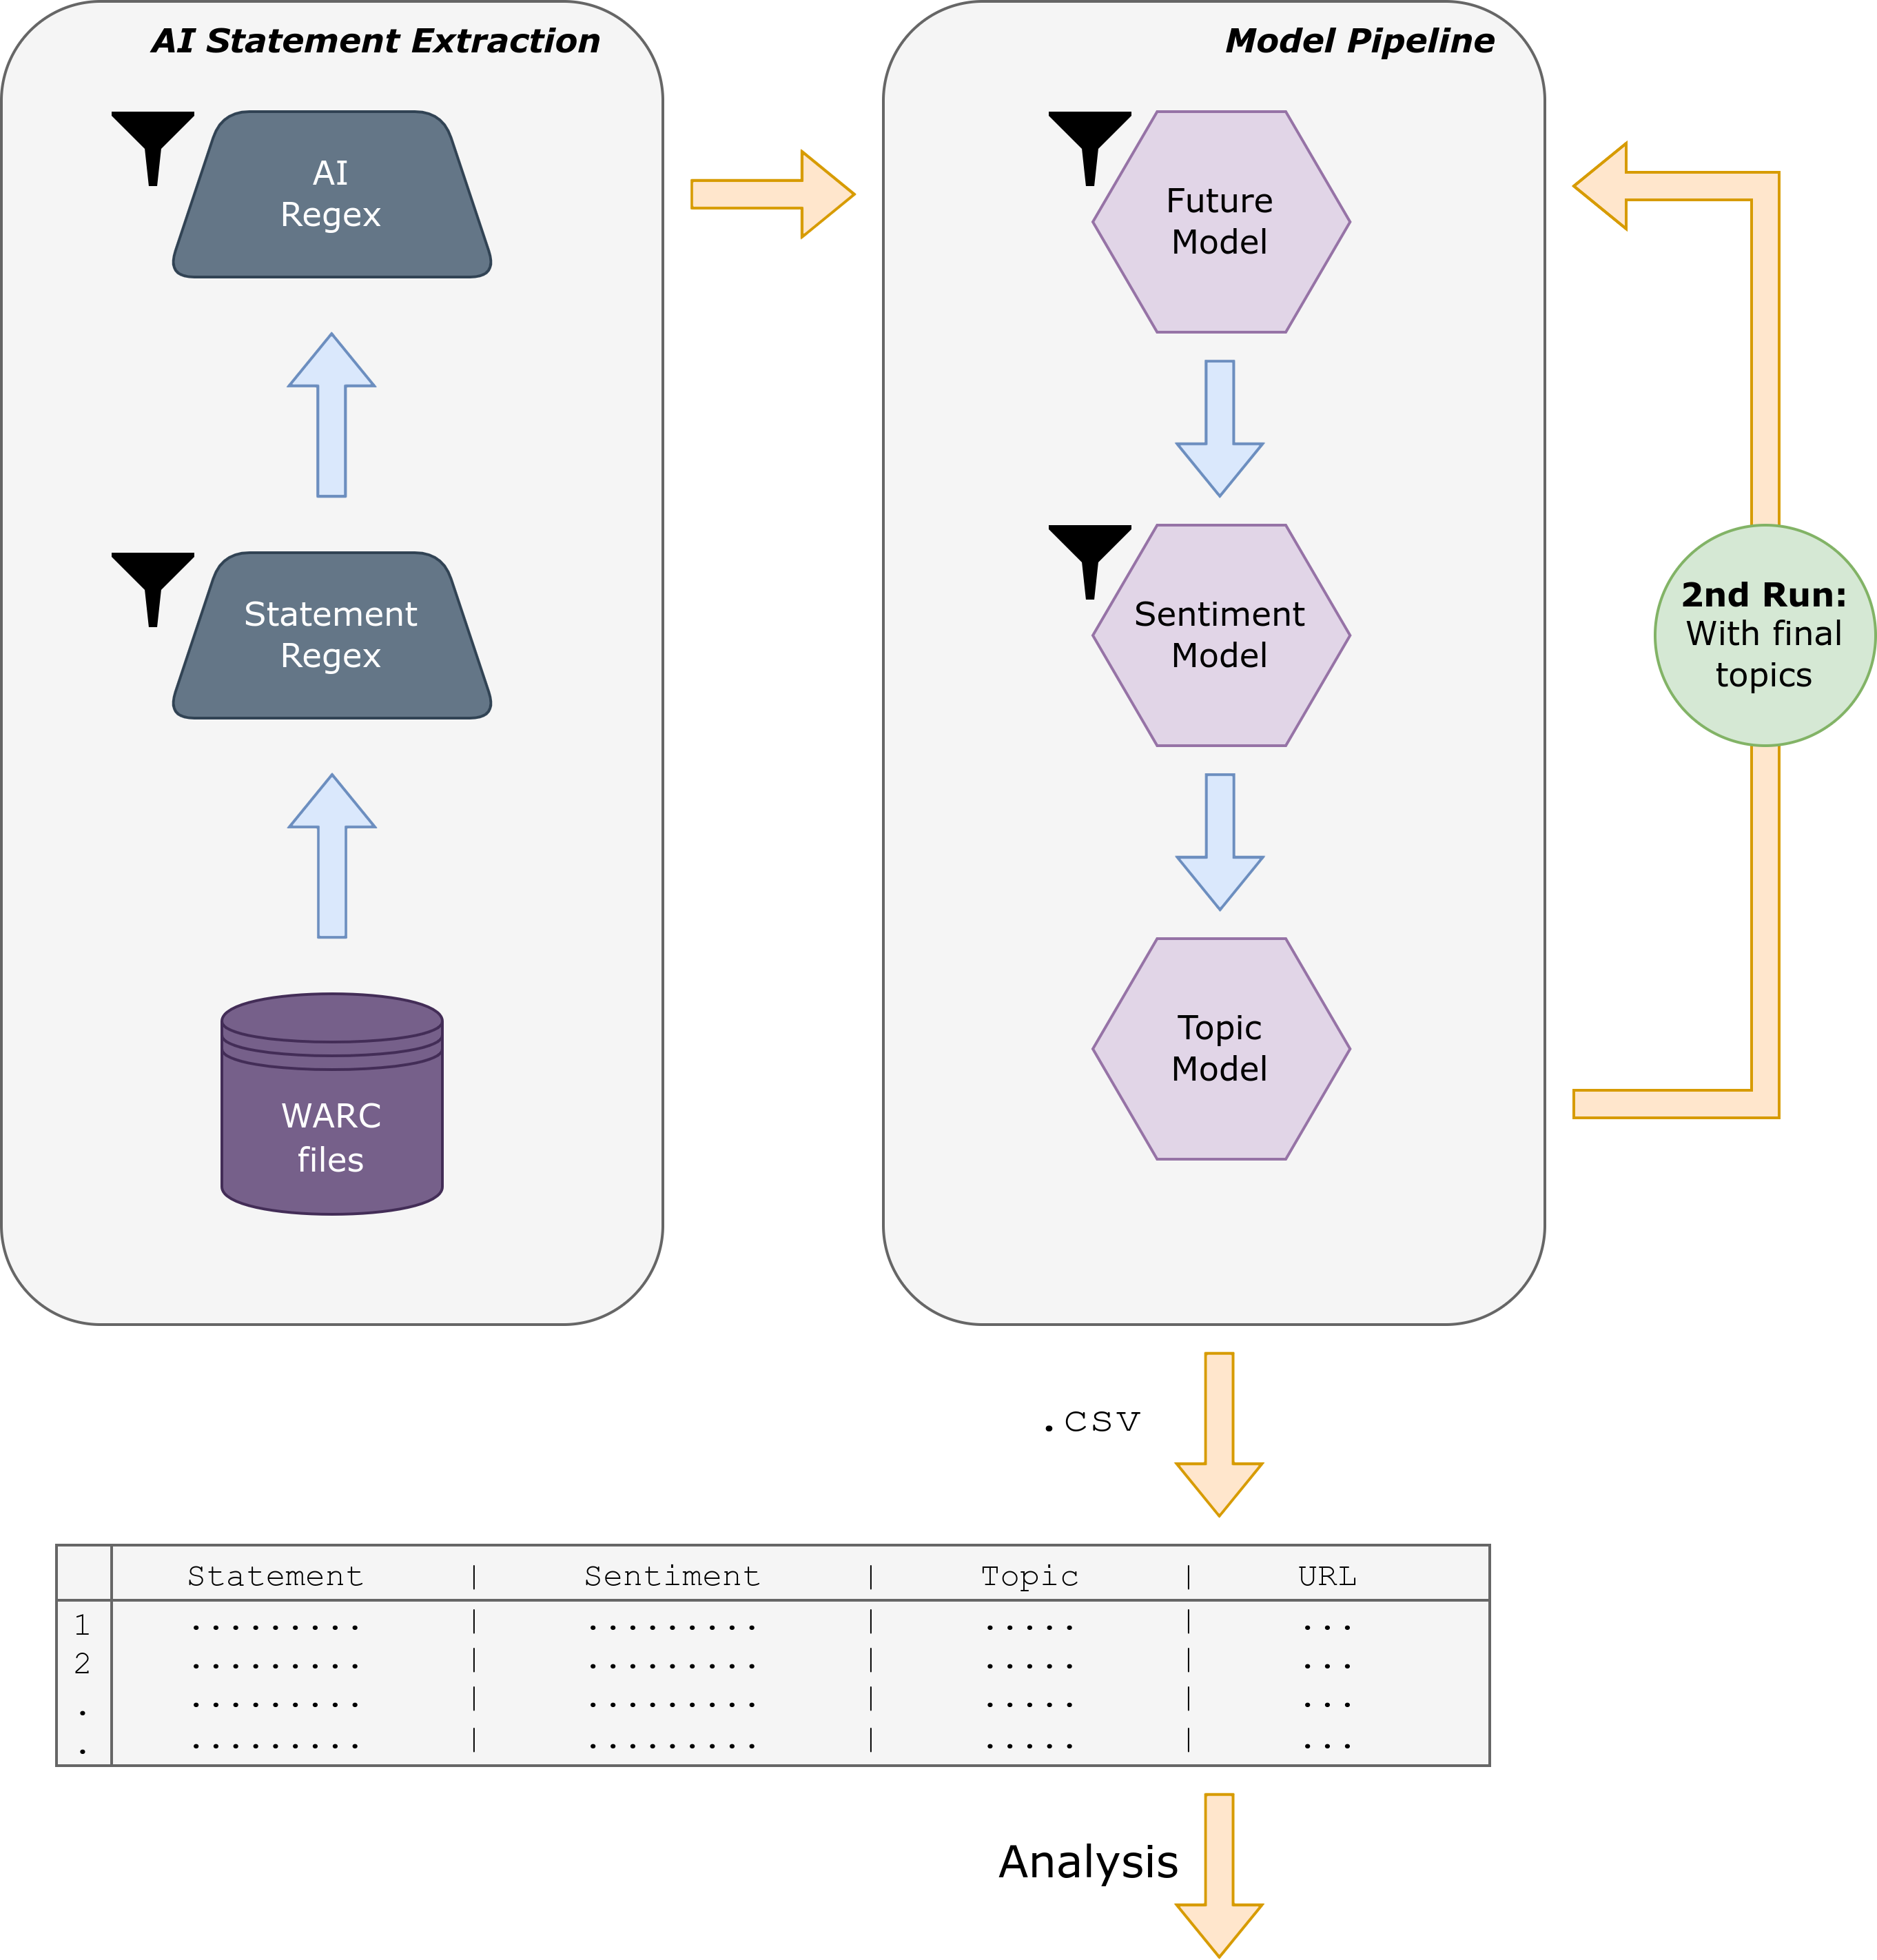
\includegraphics[width=\linewidth]{overview}
    \caption{
        The statement extraction, filter and final topic assignment process.
        AI statements are extracted from website HTMLs located inside WARC files (left part).
        The extraction process involves the application of two regexes (statement regex and AI regex).
        Statements then enter the model pipeline (left side), where they are further filtered through the future model and the sentiment model.
        The model pipeline runs two times in total. The first time the topic model assigns dummy topics.
        After the topic selection process (green circle), where we fine-tune the topic model, the model pipeline runs a second time.
        Now the topic model assigns the final topics to the statements.
        The output is a CSV file with the schema \texttt{statement|sentiment|topic|url}.
    }
    \label{fig:overview}
\end{figure}
\underline{1. WARC Data Extraction:}
\\
Initially, we outline the raw data acquisition containing AI expressions.
Since a web archive with the corresponding WARC-DL data extraction pipeline \citep{Deckers2022} was at our disposal, we utilized both.
Sentences about AI can be extracted for later processing by applying Regular Expressions (Regex) on every sentence of the data.
\\
\\
%
\underline{2. Data Transformation:}
\\
For later analysis, the data had to be converted into the required target schema, illustrated in \autoref{fig:overview}.
Therefore, we created a model pipeline which generates the final dataset with the attributes future statement, sentiment, topic, and URL.
Three sequential models are applied within this model pipeline:
\begin{itemize}
    \item Future Statements Model:\\
    This model is able to distinguish between statements about the future and all other types of statements.
On the basis of its classifications, we only extracted statements about the future.
    \item Sentiment Model:\\
A sentiment is assigned to every future statement by this model.
    \item Topic Model: \\
    Before our topic model of choice is able to assign  reasonable topics to our statements, those had to be provided to it as label candidates.
Accordingly, the Model Pipeline runs twice. In the first execution the chosen model runs with dummy topics. Based on the output, the topic selection is conducted.
For each subsequent run, the model pipeline is considered complete.
\end{itemize}%
%
The resulting dataset can then be used for analysis and interpretation.
\\
\\
\underline{3. Analysis:}
\\
For our analysis, we start with a graphical visualization.
Therefore, we decided to group all statements according to their topics so that a sentiment analysis could be conducted for each topic separately.
\\
\\
In the following sections, each step of the implementation is discussed in detail.


\subsection{WARC Data Extraction}
The Webis Group\footnote{\url{https://webis.de}} had granted us  access to 37,908 Web ARChive (WARC) files and a high-performance computer cluster on which we were able to schedule jobs.
Additionally, we decided to utilize the WARC-DL pipeline \citep{Deckers2022}, a Python software pipeline tightly coupled with the WARC endpoint, and to use the FastWARC\footnote{\url{https://resiliparse.chatnoir.eu/en/stable/man/fastwarc.html}} library for iterating over WARC records under the hood.
It enabled us to automatically extract text  from the WARC records using several customizable filters.
We made some slight modifications to the source code to make it fit our needs better.
\\
To find all statements on a website related to AI, we first built a Regex pattern to cut text from an HTML source. A second Regex pattern then extracted statements containing one or more AI keywords from this text. Since we wanted to analyze AI statements, we did not need all the text provided by a website HTML, but only full sentences of the English language. 
As it proved impossible to extract all statements with a 100\% accuracy using Regex only, we narrowed our filter down to passages which started with a capital letter and ended with a period or exclamation mark.
\\
\\
Additionally, since initial runs of the WARC-DL pipeline included large amounts of inappropriate content (including content in languages other than English), we created a whitelist to only accept the most common English language top level domains and a blacklist for filtering out domain names related to adult-content websites. 
\\
Due to problems with the cluster and WARC-DL pipeline, we could not extract all statements in one job run; jobs would suddenly stop because of connection errors or out-of-memory errors, and halt with exceptions. To overcome this issue, we separated hostnames in four groups depending on the initial hostname character: \texttt{a-h}, \texttt{i-p}, \texttt{q-x} and \texttt{yz0-9}.
This allowed us to pinpoint the problematic websites more precisely. In the end, we managed to extract data from all WARC files in group \texttt{i-p} and \texttt{yz0-9}, and most of the WARC files in groups \texttt{a-h} and \texttt{q-x}.
The final yield of the WARC data extraction stage was a total amount of 222,246 AI statements.
In the next steps, starting with the model pipeline, our objective was to further refine this initial data set.

\subsection{Model Pipeline}
\label{model-pipeline}
The model pipeline followed the WARC data extraction step and was designed to prepare our final dataset of future statements and their associated sentiment and topic labels. We performed the processing within the model pipeline on batches of 30 records each from the WARC-DL output. 
\\
First, the future model filtered out future statements from the corresponding batch. Subsequently, the chosen sentiment model assigned a sentiment to each future statement. In this step some future terms could be sorted out. This concerns the statements to which a sentiment was classified with a probability of less than 70\%. The remaining future statements received a topic. Finally, those were persisted in a CSV file.
\\
The following sections \ref{future-model} - \ref{topic-model} will go into detail about each individual model.
In this context, we describe how the future model was trained and justify our decision for the sentiment and the topic model selection.
Furthermore, we outline the choice of our topics and explain, why only those statements are kept which a sentiment with a probability above 70\% can be attributed.

\subsection{Future Model}
\label{future-model}
Since this paper focuses on analyzing statements about the future, a system for distinguishing between future statements and other expressions is required.
In this context, we decided to finetune the DistilBERT \citep{Sanh2019DistilBERTAD} base model that accomplishes this task.
Therefore, in this subsection, we thematize the collection of appropriate training data and the subsequent finetuning of the corresponding model.

\subsubsection{Training Data Set}
\label{training}
To collect suitable data for training the Future Model, we needed a balanced dataset containing statements classified as addressing the future and all other, non-future statements. We therefore adopted multiple approaches.
In order to increase diversity and reduce bias, two of our group members manually annotated 500 observations each, while the other two built an automated mechanism with subsequent verification.
\\
One of the automatized approaches involves a web crawler developed on the basis of the python library Beautiful Soup \citep{Richardson2022}.
It works by dividing the text on a page into sentences.
Subsequently, every sentence is examined for occurrence of certain terms, such as \emph{going to}, \emph{will}, \emph{won't} or \emph{'ll}.
\\
The second automated approach is a sentence extraction tool, which works similar to the web crawler in several aspects.
At the beginning, it searches the given directory for text files.
If those exist, the text is split into sentences and observed for specific expressions, as described above.
\\
To find the phrases that are not future statements, both the web crawler and the sentence extraction tool look only at the corresponding records that do not contain the previously considered expressions.
A careful manual review of all terms gathered by the automated systems was subsequently performed to remove the incorrect records.
\\
Finally, we constructed a dataset with 1,250 future statements and 1,250 other phrases that did not contain future statements.

\subsubsection{Training}
As previously described, we used the DistilBERT base model and finetuned it with the data set specified in \ref{training}.
We split the dataset of 2,500 records into a training and a test set, where the test set contained 20\% of the records.
From the training set we further split 20\% for validation data.
\\
After only two epochs the training ended with an accuracy over 96\% as displayed in \autoref{future-model-train}.
\\
Following, we tested the model on our test set containing 500 records never seen by the model and achieved an accuracy of 93.8\%, as seen in the confusion matrix in \autoref{fig:cm}.


\subsection{Sentiment Model}
In order to assign sentiments to future statements for later analysis, we decided to select a pre-trained model.
The chosen sentiment model is the SentimentAnalyzer of the open-source library pysentimiento \citep{perez2021pysentimiento}, which was further trained on about 40,000 tweets.
It uses the BERTweet \citep{bertweet} model as a base model, pre-trained on English language tweets.

\subsubsection{Evaluation}
To evaluate the SentimentAnalyzer, we annotated 604 future statements, previously used for training the future model, as negative, positive or neutral and received an accuracy of about 65\%.
\\
We then analyzed all misclassified statements and noticed that some of them could not be assigned impartially to one of the three categories.
An example is \emph{``AI will reinvent how we think about education''}.
In the case of this sentence, we disagreed on whether we should value the sentence as neutral or positive and decided to use the neutral label.
However, this statement was given a positive rating by the model.
On closer examination of the statements that were labeled differently by us and by the model, we found over 90\% of the labels given by the model to be valid, if these annotations had a probability of correctness over 70\%.
For this reason we decided to only keep statements about the future which the sentiment model had annotated with a confidence above 70\%.

\subsection{Topic Model}
\label{topic-model}
\begin{figure}[t]
    \centering
    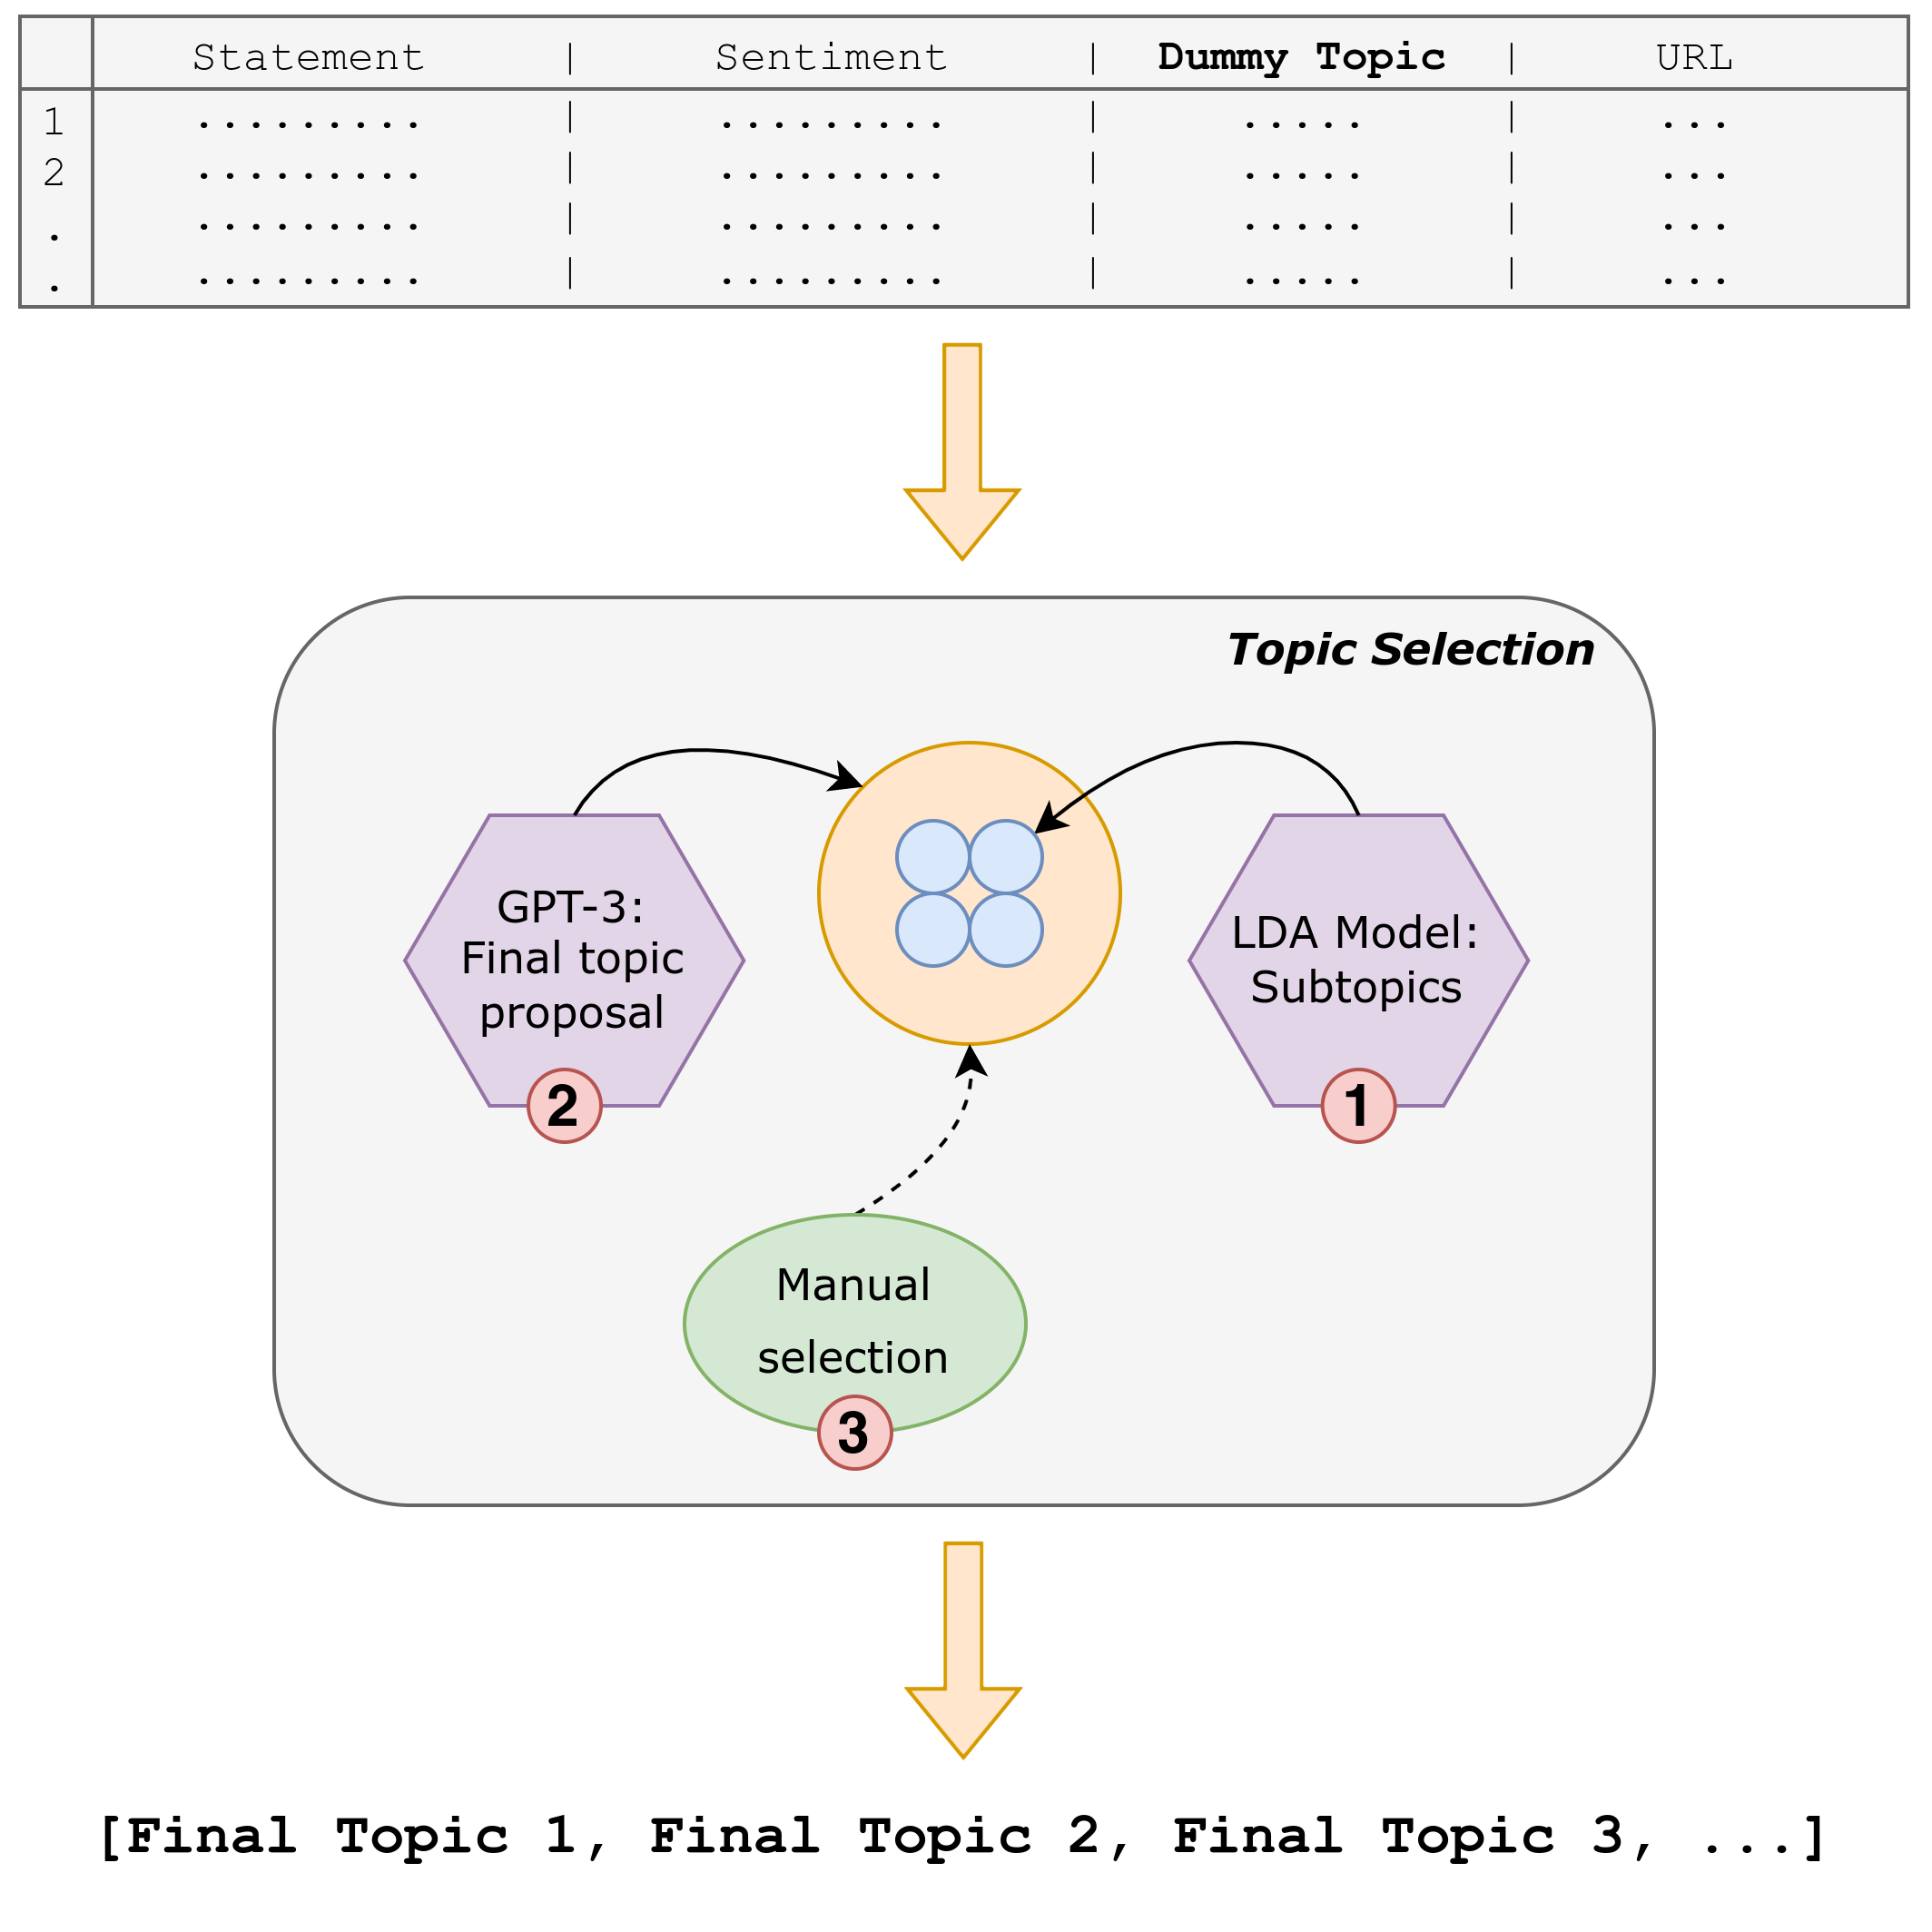
\includegraphics[width=\linewidth]{topic_selection}
    \caption{
        The three steps of topic selection.
        First, the LDA Model generates a set of subtopics for a topic cluster.
        In this example, there are four subtopics (small blue circles).
        Then, GPT-3 proposes a possible general topic for the subtopic set (large yellow circle).
        Lastly, we either pick this final topic as proposed, or replace it with a more suitable one from the same category, e.g. \texttt{level} would become \texttt{gaming}.
    }
    \label{fig:topic_selection}
\end{figure}
For assigning topics to the future statements we employed the bart-large-mnli model from Facebook, which was pre-trained on the MultiNLI \citep{N18-1101} dataset, which consists of 433,000 pairs of sentences annotated with textual supplementary information. The bart-large-mnli is a natural language processing model based on the technique of \citet{yin2019benchmarking} utilizing pre-trained NLI models as ready-to-use zero-shot sequence classifiers.
The approach involves specifying the sequence for classification as an NLI prerequisite and then constructing a hypothesis of every possible label candidate.
Afterwards probabilities of agreement and contradictions are transformed into annotation probabilities.
Before we were able to use the bart-large-mnli, however, it was necessary to define the topics, which could be assigned to every statement by this model.
For instance, to verify whether a sentence was a political or a technological statement, we could provide the model with the label candidates: \emph{politics} and \emph{technology}. Then the model would apply one of the labels to the sentence.
The following section describes our topic selection approach in detail.

\subsubsection{Topic Discovery with LDA}
\label{lda}
For analyzing the overarching topics within our future statements, we used Latent Dirichlet Allocation (LDA). LDA is a subtype of the Dirichlet Process Mixture Models (DPMMs), a set of non-parametric, “fully-Bayesian” unsupervised clustering models which are commonly used for topic cluster analysis. DPMMs use a stochastic process to generalize the Dirichlet distribution (the conjugate prior for a categorical or multinomial distribution) for infinitely many categories \citep{li2019tutorial}.
Applied to NLP, a Latent Dirichlet Allocation model clusters observations into unobserved groups of related data. It has the advantage of following a generative process that is immune to overfitting with increasing size of the data corpus and can be scaled to a data cluster in machine learning \citep{pritchard2000inference}.
\\
\\
We preprocessed our dataset for LDA.
From there on, we created bigrams (sets of two words) from the tokens and employed a Word2Vec model to select only the most frequently occurring ones.
Afterwards, bigrams that occurred in more than 60\% statements and less than 20 of the documents were filtered out. The remaining bigram candidates were fed into an LDA model, returning clusters of related topics. To label each cluster with a matching headline or cluster name, we used OpenAI’s GPT-3 (text-davinci-002) to turn suggestions of cluster names.
\\
Inspired by these suggestions, we chose topic names that we considered the best fit for for every cluster of topics.
Eventually, with this approach we received the following headings for our Topic Model: search engine, finance, transhumanism, machine human interface, social media, search engine, and natural language technologies.


\subsection{Analysis}
For the analysis of the previously created dataset in \ref{model-pipeline}, we focused on the attributes topic, subtopic, network, and sentiment of each tuple.
Since the future dataset generated by the Model Pipeline only captured the topic or category of a future statement and the sentiment attribute, we included further subtopics.
To accomplish this, we proceeded as described in section \ref{lda}.
Consequently, the resulting data for every statement contained not only a topic but also a subtopic.
This way we intended to analyze each future statement category in more detail.
To accomplish this we extracted the original subcategory list of each topic utilizing the LDA model and combined these lists to a single one. We aimed to find a subtopic for almost every statement.
Therefore, we checked whether a statement contained a subtopic from the list and selected the first one.
To obtain the most suitable assignment of subtopics to statements, we maintained the order of these subcategories within each original list.
In conclusion, the more meaningful statement subtopics found by the LDA model were prioritized. Sentences that did not contain any of this subtopics were marked as 'undefined'.
This way, we were able to obtain the average sentiment scores for each theme and subcategory.
\\
\\
Furthermore, we added a number to every statement, mapped to every statement for a later sentiment score calculation. To negatively perceived sentences we assigned a \texttt{–1}, while positively labeled terms receive a \texttt{1}. Finally, every statement containing a neutral sentiment obtains a \texttt{0}.

\section{Results}

\section{Discussion}

\subsection{Results}
Our results reveal a slightly positive outlook of people on future of AI.
Interestingly, two thirds of our filtered statements were neutral, which, together with the nature of our top domain sources, suggests a large proportion of texts coming from academic or unbiased texts rather than strong opinions.
The presence of about twice as many positively compared to negatively sentences and thereby a rather hopeful outlook into the future, may also be influenced by the optimism bias, which is when humans tend to overestimate the likelihood of positive events and underestimate that of negative \citep{sharot2011optimism}.
These findings also align with a large-scale study made by Google researchers on the public opinion regarding the long-term impact of AI on society (Kelley et al., 2021).
This study, which surveyed people from eight English and non-English speaking countries, shows a clear dominance of neutral perceptions in English-speaking countries (USA: 53\%, Australia: 57\%, Canada: 56\%) and a greater proportion of positive sentiments (USA: 21\%, Australia: 18\%, Canada: 20\%) than negative (USA: 17\%, Australia: 14\%, Canada: 15\%).
Intriguingly, respondents from emerging economies such as Brazil, India and Nigeria exhibit far more optimistic opinions on the future of AI (BR: 38\%, IN: 51\%, NI: 37\%), a finding that has been repeatedly confirmed in a recent survey by the World Economic Forum \citep{Markovitz2022}.
This difference may be due to these countries’ younger and generally more optimistic population, which may view AI as an essential opportunity for leapfrogging \citep{zhenmin2019frontier}.
While we filtered our statements for English-speaking websites only, the prevalence of English as the world’s lingua franca must have led to the inclusion of opinions and statements from non-English speaking people.
This may explain the slight skew towards positive sentiments in our data compared to sentiments from the USA, Australia and Canada from \citet{kelley2021exciting}.
Comparing our topic clusters with the dichotomies of hopes and fears by \citet{cave2019}, we can only find a weak overlap between the data.
\emph{machine human interface} and \emph{transhumanism} well match the authors’ first category of Immortality and Inhumanity.
Interestingly, all subtopics within these clusters were labelled either neutral or positive, with those from \emph{transhumanism} even displaying the most positive sentiments.
The only subtopic receiving a negative label when compared to the overall sentiment mean of 0.1 (\highlight{Appendix XXX}) is \emph{autopilot} from the \emph{machine human interface} cluster, suggesting the main concern to be losing conscious control by the use of such interfaces in the future.
From this, we conclude a disproportionate number of opinions in favor of \emph{transhumanism} and a machine-enabled future in relation to opinions highlighting the possible (existential) risks and dangers to our ``human'' identity.
The \emph{natural language technology} cluster in turn may point towards applications of such technologies that make life easier, such as Amazon’s Alexa, thereby fitting the category of Ease and possibly Gratification.
Yet, the corresponding counterparts in the dichotomies are hard to find in our clusters, where the only negatively labelled subtopics exist in the gaming cluster.
This aspect can be explained by the increasing prevalence of AI-mediated systems in games, from non-playable characters (which can include \emph{enemies}, a highly negative subtopic) to iterative game improvement and graphical enhancement \citep{anandrise}.
While the latter two examples provide advantages for the gamer, it may be that the idea of an AI as the enemy predominates since this is the primary noticeable direct touchpoint between the user and an AI.
Furthermore, there are no clusters that we consider well-fitting for \citet{cave2019} category Dominance and Uprising, which, curiously, is a category commonly discussed by popular figures such as the late Stephen Hawking \citep{hawking2014transcendence}.
Overall, it rather that our clusters center around applications of artificial intelligence.
This is further demonstrated by the fact that several subtopics repeat within clusters (\highlight{Figure XXX}). For instance, \emph{autopilot} is present within the \emph{machine human interface}, \emph{natural language processing}, \emph{finance}, \emph{search engine}, \emph{social media}, and \emph{transhumanism} clusters.
Other repeated subtopics include \emph{data}, \emph{supercomputer}, \emph{computer}, \emph{intelligence}, \emph{recognition}, and \emph{machine}. Together with the slightly positive but largely neutral overall sentiment, which suggests that people speak mainly rationally about the future of AI, we reason that discussions center primarily around areas of application of AI technology instead of opinionated positions about its benefits and risks.

\subsection{Topic Assignment}
\label{topics}
As described in section \ref{results} the most statements are assigned with the \emph{machine human interface} topic.
This is not surprising, since technical sources clearly dominate our websites.
Technological systems often require human operation and contain a corresponding interface as an implicit feature.
Also search engines often need the handling from the outside.
For this reason, many of these search engine related phrases end up in this category instead of in the search engine topic.
Since search engines also correspond to natural language systems, they are often assigned to the category \emph{natural language technology}.
To avoid this, more distinct generic terms for topics should have been chosen.
This issue also arises in the field of \emph{human machine interface}.
Statements that describe a friendly AI are grouped in this category.
We would expect this kind of sentences in \emph{transhumanism}.
The reason for this could be the categpry name, since it combines the terms human and machine.
\\
\emph{computer vision}, \emph{natural language technology}, \emph{social media}, \emph{transhumanism} and \emph{human machine interface} contain many statements that do not fit the corresponding topic.
Whereas this appears quite random for \emph{natural language technology} and \emph{human machine interface}, since we did not define suitable topics for these sentences.
In \emph{computer vision} many sentences end up containing words like scan, look, see.
But these do not actually refer to the topic.
Similarly \emph{social media} includes  statements with the word fans, even if this sentence is about attending a soccer match.
But also in this category are plenty of randomly assigned statements.
Nevertheless, the categories \emph{computer vision} and \emph{natural language technology} also contain appropriate phrases.
The quality of these subjects is mixed.
\emph{human machine interface} consists of far too many terms that do not fit to this topic.
A possible solution for such random assignments could be to add the generic category \emph{others}.
Furthermore, it should be considered whether the category human machine interface is actually useful.
It does not seem specific enough to narrow down a particular topic.
\\
The Topic Model seems to assign the \emph{research computing} category to statements more reliably.
Nevertheless, it is noticeable that educational topics that cannot be associated with research and hardware or software are also grouped under this theme.
Sentences regarding technical topics, which have no connection with research, also often fall into this category.
However, in the end it is a matter of interpretation whether these statements do not fall under \emph{research computing}.
\\
Finally, there are also topics that seem to be correctly assigned to their statements for the majority of the time.
The corresponding categories are finance and gaming.
This could be an indication that the model is not suitable for too specific technical terms.
Providing more common topics contained in the everyday english language use, could result in a more reliable topic annotation.

\subsection{Website Examination}
The final data set, produced by the model pipeline, contains the URL for every AI future statement.
\autoref{Top-Domains} presents the domains that are mostly occurring in this final data set.
When examining the main domains, these appear relatively  diversified.
A website dealing with phylosophical questions on the topic of AI is included (\texttt{lesswrong.com}).
Following this, there are three sites from the field of gaming (\texttt{acceleratingfuture.com}, \texttt{mugenguild.com}, \texttt{slightlymagic.net}).
Also, the blog of the department of defense is contained among these domains dealing with the research of defence and military needs (\texttt{dodsbir.net}).
A store with speech recognition devices is also available (\texttt{knowbrainer.com}).
Nevertheless a number of scientific blogs on AI-related topics are also include, which are lead by researchers or from the tech industry.
Latter are mostly data scientists.
Considering the other domains, many scientific websites as well as websites about gaming are also very abundant.
Thus, rather the future statements were expressed by people from AI related fields.
This could mean that this topic has a lower role in the general population and thus it is dealt very little with AI-specific topics in the public society.
New discoveries could be made by observing domains containing statements from the last few months were used.
More people might feel affected by the latest developments in this area.
Consequently, there could be more blogs with people from other sectors who would exchange opinions about these developments.
%%%%%%%%%%%%%%%%%%%%%%%%%%%%%%%%%%%%%%%%%%%%%%%%%%%%%%%%%%%%%%%%%%%%%%%%%%%%%%%%%%%%%%%%%%%%%%%%%%%%%%%%%%%%%%%%%%%%%%%%%%%%%%%%%%%%%%%%%%%%%%%%%%%%%%
%%%%%%%%%%%%%%%%%%%%%%%%%%%%%%%%%%%%%%%%%%%%%%%%%%%%%%%%%%%%%%%%%%%%%%%%%%%%%%%%%%%%%%%%%%%%%%%%%%%%%%%%%%%%%%%%%%%%%%%%%%%%%%%%%%%%%%%%%%%%%%%%%%%%%%
\begin{table}
    \setlength\tabcolsep{2pt} % let LaTeX compute intercolumn whitespace
    \centering
    \captionsetup{size=footnotesize}
    \resizebox{\columnwidth}{!}{%
    %\begin{tabular*}{\columnwidth}{@{\extracolsep{\fill}}%
    %%%%%%%%%%%%%%%%%%%%%%%%%%%%%%%%%%%%%%%%%%%%%%%%%%%%%%%%%%%%%%%%%%%%%%%%%%%%%%%%%%%%%%%%%%%%%%%%%%%%%%%%%%%%%%%%%%%%%%%%%%%%%%%%%%%%%%%%%%%%%%%%%%%%%%
    \begin{tabular}{rll}
        \toprule
        \textbf{AI statements} & \textbf{Website} & \textbf{Description} \\
        \midrule
        \multirow{2}{*}{210\quad} & \multirow{2}{*}{lesswrong.com}          & Philosophical blog \\
                                  &                                         & about AI developments \\
        \addlinespace[0.7em]
        \multirow{2}{*}{198\quad} & \multirow{2}{*}{arcengames.com}         & Page of an indie \\
                                  &                                         & game developer \\
        \addlinespace[0.7em]
        \multirow{2}{*}{182\quad} & \multirow{2}{*}{acceleratingfuture.com} & Blog about perspectives \\
                                  &                                         & and emerging technologies \\
        \addlinespace[0.7em]
        \multirow{2}{*}{156\quad} & \multirow{2}{*}{heatonresearch.com}     & Blog of a data \\
                                  &                                         & scientist \\
        \addlinespace[0.7em]
        \multirow{2}{*}{106\quad} & \multirow{2}{*}{dodsbir.net}            & Research blog of the \\
                                  &                                         & department of defense \\
        \addlinespace[0.7em]
        \multirow{2}{*}{76\quad}  & \multirow{2}{*}{kdnuggets.com}          & Blog of data scientists for \\
                                  &                                         & analytics and machine learning \\
        \addlinespace[0.7em]
        \multirow{2}{*}{71\quad}  & \multirow{2}{*}{knowbrainer.com}        & Shop containing speech \\
                                  &                                         & recognition devices\\
        \addlinespace[0.7em]
        {58\quad}                 & mugenguild.com                          & 2D fighting game \\
        \addlinespace[0.7em]
        {52\quad}                 & aidreams.co.uk                          & Robotics and AI blog\\
        \addlinespace[0.7em]
        \multirow{2}{*}{51\quad}  & \multirow{2}{*}{slightlymagic.net}      & Rules Engine for the game \\
                                  &                                         & ``Magic: the Gathering'' \\
        \bottomrule
    \end{tabular}
    }
\caption{\label{Top-Domains}
Top Domains
}
\end{table}
%%%%%%%%%%%%%%%%%%%%%%%%%%%%%%%%%%%%%%%%%%%%%%%%%%%%%%%%%%%%%%%%%%%%%%%%%%%%%%%%%%%%%%%%%%%%%%%%%%%%%%%%%%%%%%%%%%%%%%%%%%%%%%%%%%%%%%%%%%%%%%%%%%%%%%
%%%%%%%%%%%%%%%%%%%%%%%%%%%%%%%%%%%%%%%%%%%%%%%%%%%%%%%%%%%%%%%%%%%%%%%%%%%%%%%%%%%%%%%%%%%%%%%%%%%%%%%%%%%%%%%%%%%%%%%%%%%%%%%%%%%%%%%%%%%%%%%%%%%%%%
\subsection{Project Limitations}

Since we had a limited time for this project, there are some aspects where we would have liked to continue our work.
From a technical point of view, we would have preferred to spend additional time on labelling more data for the sentiment model.
Thus, it could have been possible to finetune this model as well.
With our current approach, we only keep the AI future predictions if the sentiment model makes a prediction with a certainty of more than 70\%.
This results in the loss of a few additional statements that we would have available for analysis.
\\
Investing more time in topic selection would also be beneficial.
Therefore, it might be reasonable to manually evaluate our statements with the corresponding topics with a subsequent performing of a another topic selection.
Furthermore, better results can be achieved by finetuning the topic model.
\\
Unfortunately, the location containing the corresponding date on the website does not contain the corresponding date is not consistent.
Accordingly, we would have needed more time for the date extraction.
Providing a year for each statement could illustrate how the perception of a certain topic in the field of AI has changed over time.
Having insights about such trends, allows monitoring the developments in cultural perceptions over time periods.
\\






\section{Conclusion}


% Entries for the entire Anthology, followed by custom entries
\bibliography{anthology,custom}

\onecolumn
\appendix
\section{Data Set Card: Future Statements}
The english language data set contains 2500 statements.
50\% of the relate to future events and 50\% of which relate to non-future events.
The statements were collected manually and programmatically from several websites and datasets.
The sole purpose of this data set was to fine tune the distilbert-base-uncased model into our distilbert-base-future model.
The data set is available on huggingface (\url{https://huggingface.co/datasets/fidsinn/future-statements}).
\\
\\
\textbf{Composition}
\\
\\
The instances are represented by single-/ or multi-sentence statements from following sources (unequally distributed):
%
\begin{itemize}
    \item \url{http://www.kaggle.com/unitednations/un-general-debates}
    \item \url{http://data.world/ian/united-nations-general-debate-corpus}
    \item \url{http://gadebate.un.org/}
    \item \url{http://dataverse.harvard.edu/dataset.xhtml?persistentId=doi:10.7910/DVN/0TJX8Y}
    \item \url{http://www.wsj.com/}
    \item \url{http://www.vox.com/}
    \item \url{http://futechblog.com/}
    \item \url{http://www.weforum.org/}
    \item \url{http://wired.com/}
    \item \url{http://openai.com/blog/}
    \item \url{http://techcrunch.com/}
    \item \url{http://futurism.com}
\end{itemize}
%
\textbf{Annotation}
%The label is represented by the 'future'-column:
\begin{itemize}
    \item 0: No future statement
    \item 1: future statement
\end{itemize}%

\section{Model Card: Future Statement Model}
This model is a finetuned on 2500 expressions, which contained 1250 future statements. distilbert-base-uncased serves as a base model
\\
\\
%
\textbf{Model Description}
%
\begin{itemize}
    \item Huggingface name: distilbert-base-future
    \item Creation Date: 11/08/22
    \item Version: 1.0
    \item model type: text classification
\end{itemize}%
%
\textbf{Intended Use \& Limitations}
%
\begin{itemize}
    \item The primary intended use is the classification of input into a future or non-future sentence/statement.
    \item The model is primarily intended to be used by researchers to filter or label a large number of sentences according to the grammatical tense of the input.
\end{itemize}%
%
\textbf{Hyperparameters}
\\
\\
The following hyperparameters were used during training
\begin{itemize}
    \item optimizer:
    name: Adam, learning\_rate: 5e-05, decay: 0.0, beta\_1: 0.9, beta\_2: 0.999, epsilon: 1e-07, amsgrad: False
    \item training\_precision: float32
\end{itemize}%
\label{sec:appendix}
%
\textbf{Training Results}
\\
For finetuning, we have 80\% of of records from our self-annotated future-tatements dataset. This corresponds to 2000 records.
The remaining 500 will be used to test the final distilbert-base-future model
\\
%%%%%%%%%%%%%%%%%%%%%%%%%%%%%%%%%%%%%%%%%%%%%%%%%%%%%%%%%%%%%%%%%%%%%%%%%%%%%%%%%%%%%%%%%%%%%%%%%%%%%%%%%%%%%%%%%%%%%%%%%%%%%%%%%%%%%%%%%%%%%%%%%%%%%%
%%%%%%%%%%%%%%%%%%%%%%%%%%%%%%%%%%%%%%%%%%%%%%%%%%%%%%%%%%%%%%%%%%%%%%%%%%%%%%%%%%%%%%%%%%%%%%%%%%%%%%%%%%%%%%%%%%%%%%%%%%%%%%%%%%%%%%%%%%%%%%%%%%%%%%
\begin{table}[ht]
    \scriptsize
    \setlength\tabcolsep{10pt} % let LaTeX compute intercolumn whitespace
    \footnotesize\centering
    \begin{tabular}{ccccc}
        \toprule
        \textbf{Epoch} & \textbf{Train Loss} & \textbf{Train Accuracy} & \textbf{Val. Loss} & \textbf{Val. Accuracy} \\
        \midrule
        0 & 0.3816 & 0.8594 & 0.1547 & 0.9475 \\
        1 & 0.1142 & 0.9613 & 0.1272 & 0.9625 \\
        \bottomrule
    \end{tabular}
    \caption{\label{future-model-train}
    Training Results
    }
\end{table}
%%%%%%%%%%%%%%%%%%%%%%%%%%%%%%%%%%%%%%%%%%%%%%%%%%%%%%%%%%%%%%%%%%%%%%%%%%%%%%%%%%%%%%%%%%%%%%%%%%%%%%%%%%%%%%%%%%%%%%%%%%%%%%%%%%%%%%%%%%%%%%%%%%%%%%
%%%%%%%%%%%%%%%%%%%%%%%%%%%%%%%%%%%%%%%%%%%%%%%%%%%%%%%%%%%%%%%%%%%%%%%%%%%%%%%%%%%%%%%%%%%%%%%%%%%%%%%%%%%%%%%%%%%%%%%%%%%%%%%%%%%%%%%%%%%%%%%%%%%%%%
%
%
\\
\textbf{Framework versions}
\begin{itemize}
    \item Transformers 4.18.0
    \item Tensorflow 2.8.0
    \item Tokenizers 0.12.1
\end{itemize}%
%
\pagebreak
\textbf{Test Set Results}
\begin{figure}[h]
    \centering
    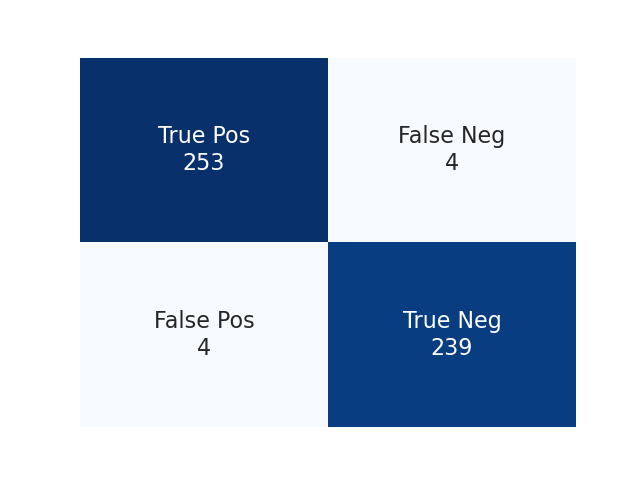
\includegraphics[width=0.5\textwidth]{cm}
    \caption{
        Dummy caption.
    }
    \label{fig:cm}
\end{figure}

\section{Remaining Figures}
\begin{figure}[h!]
    \centering
    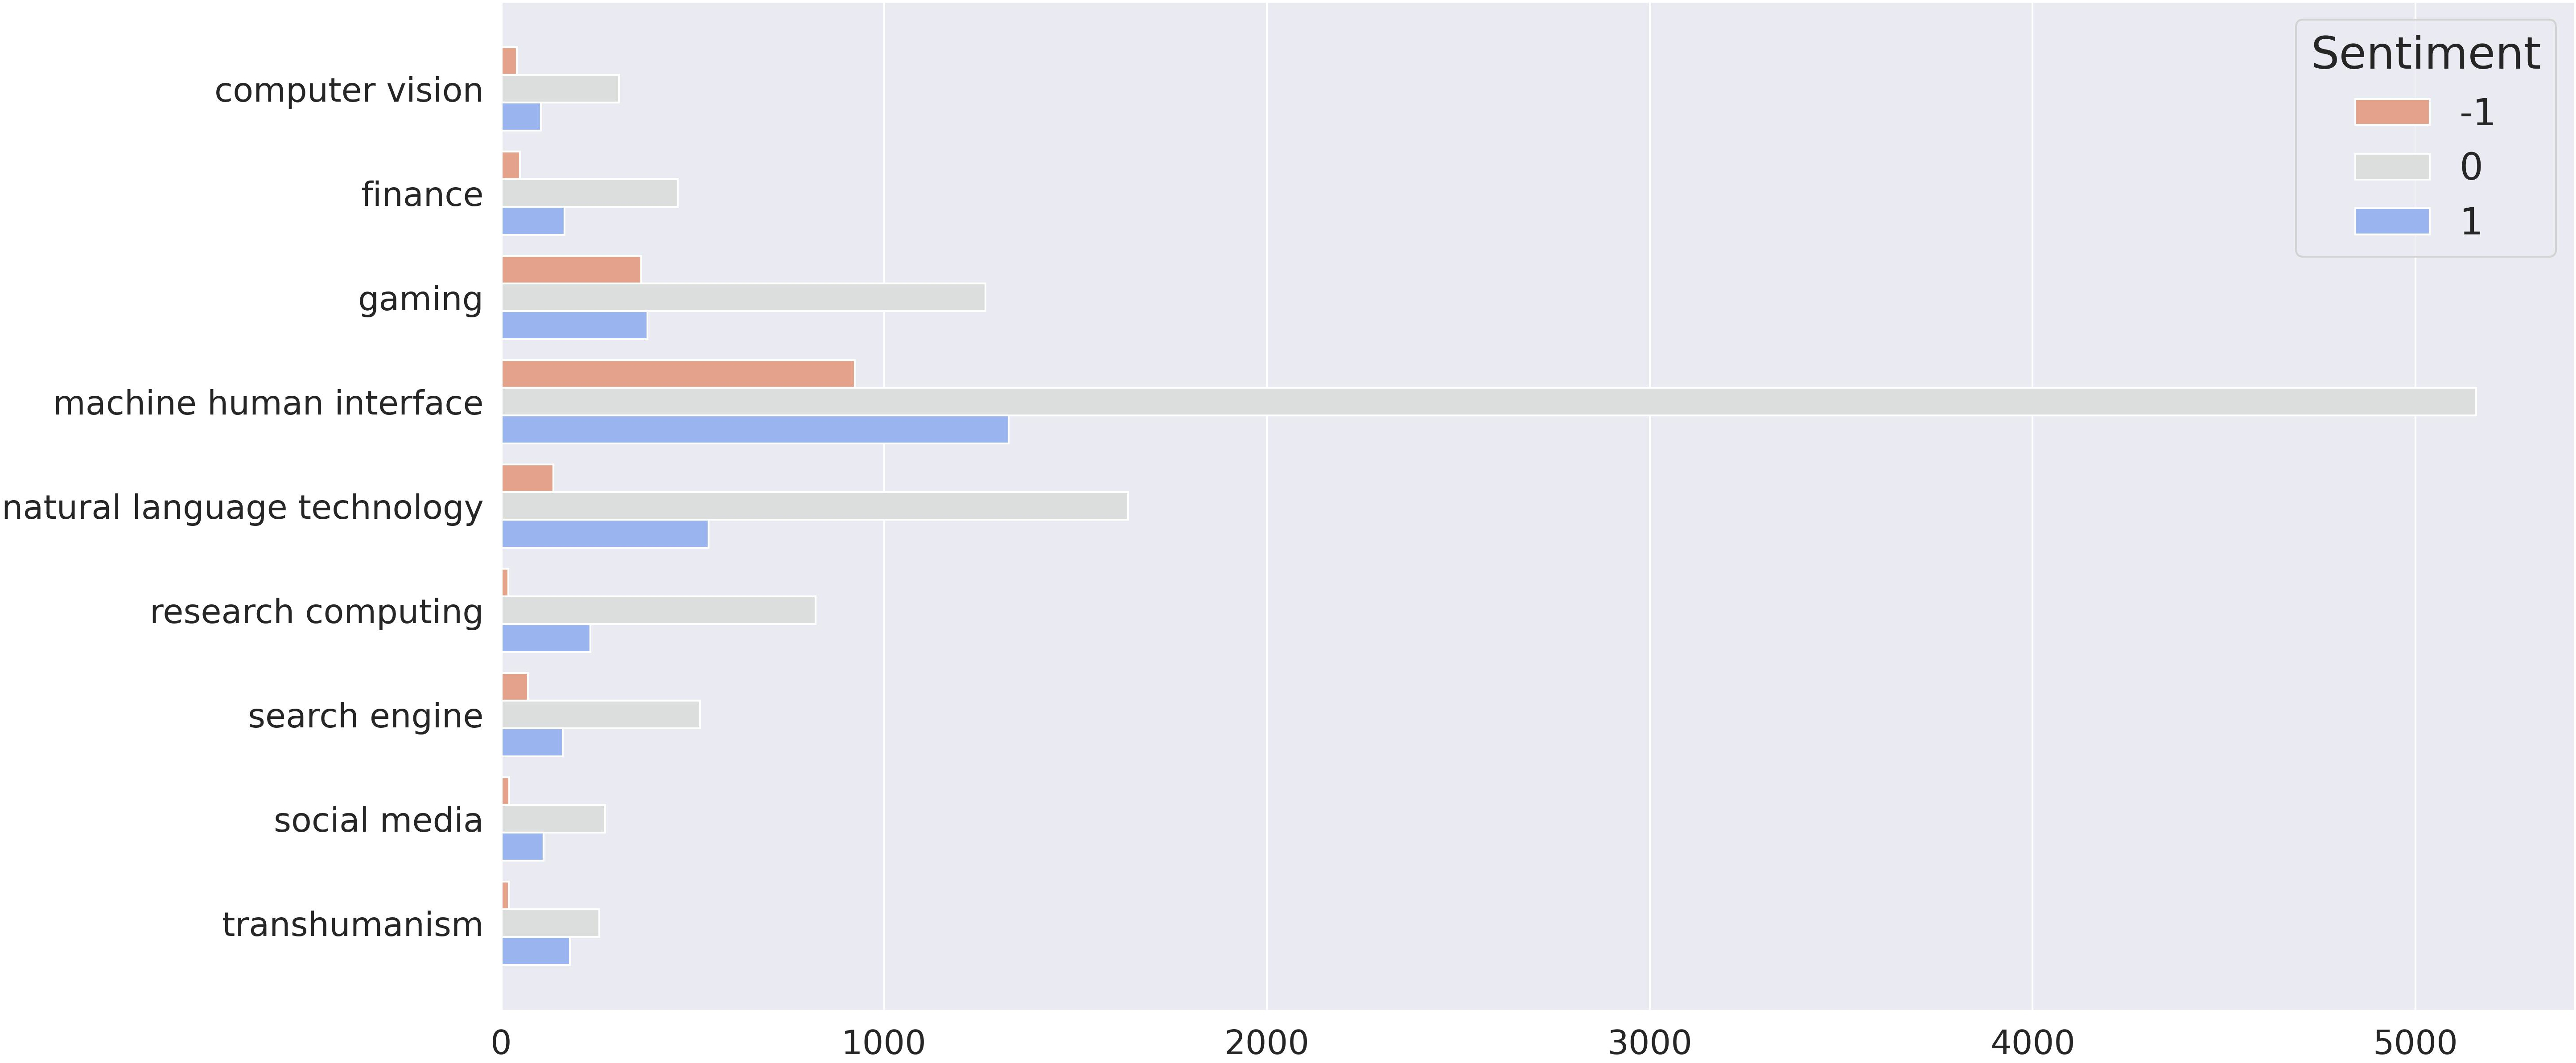
\includegraphics[width=\textwidth]{bar_topics}
    \caption{
        Dummy caption.
        Dummy caption.
        Dummy caption.
        Dummy caption.
        Dummy caption.
        Dummy caption.
        Dummy caption.
        Dummy caption.
        Dummy caption.
        Dummy caption.
        Dummy caption.
        Dummy caption.
        Dummy caption.
        Dummy caption.
        Dummy caption.
    }
    \label{fig:bar_topics}
    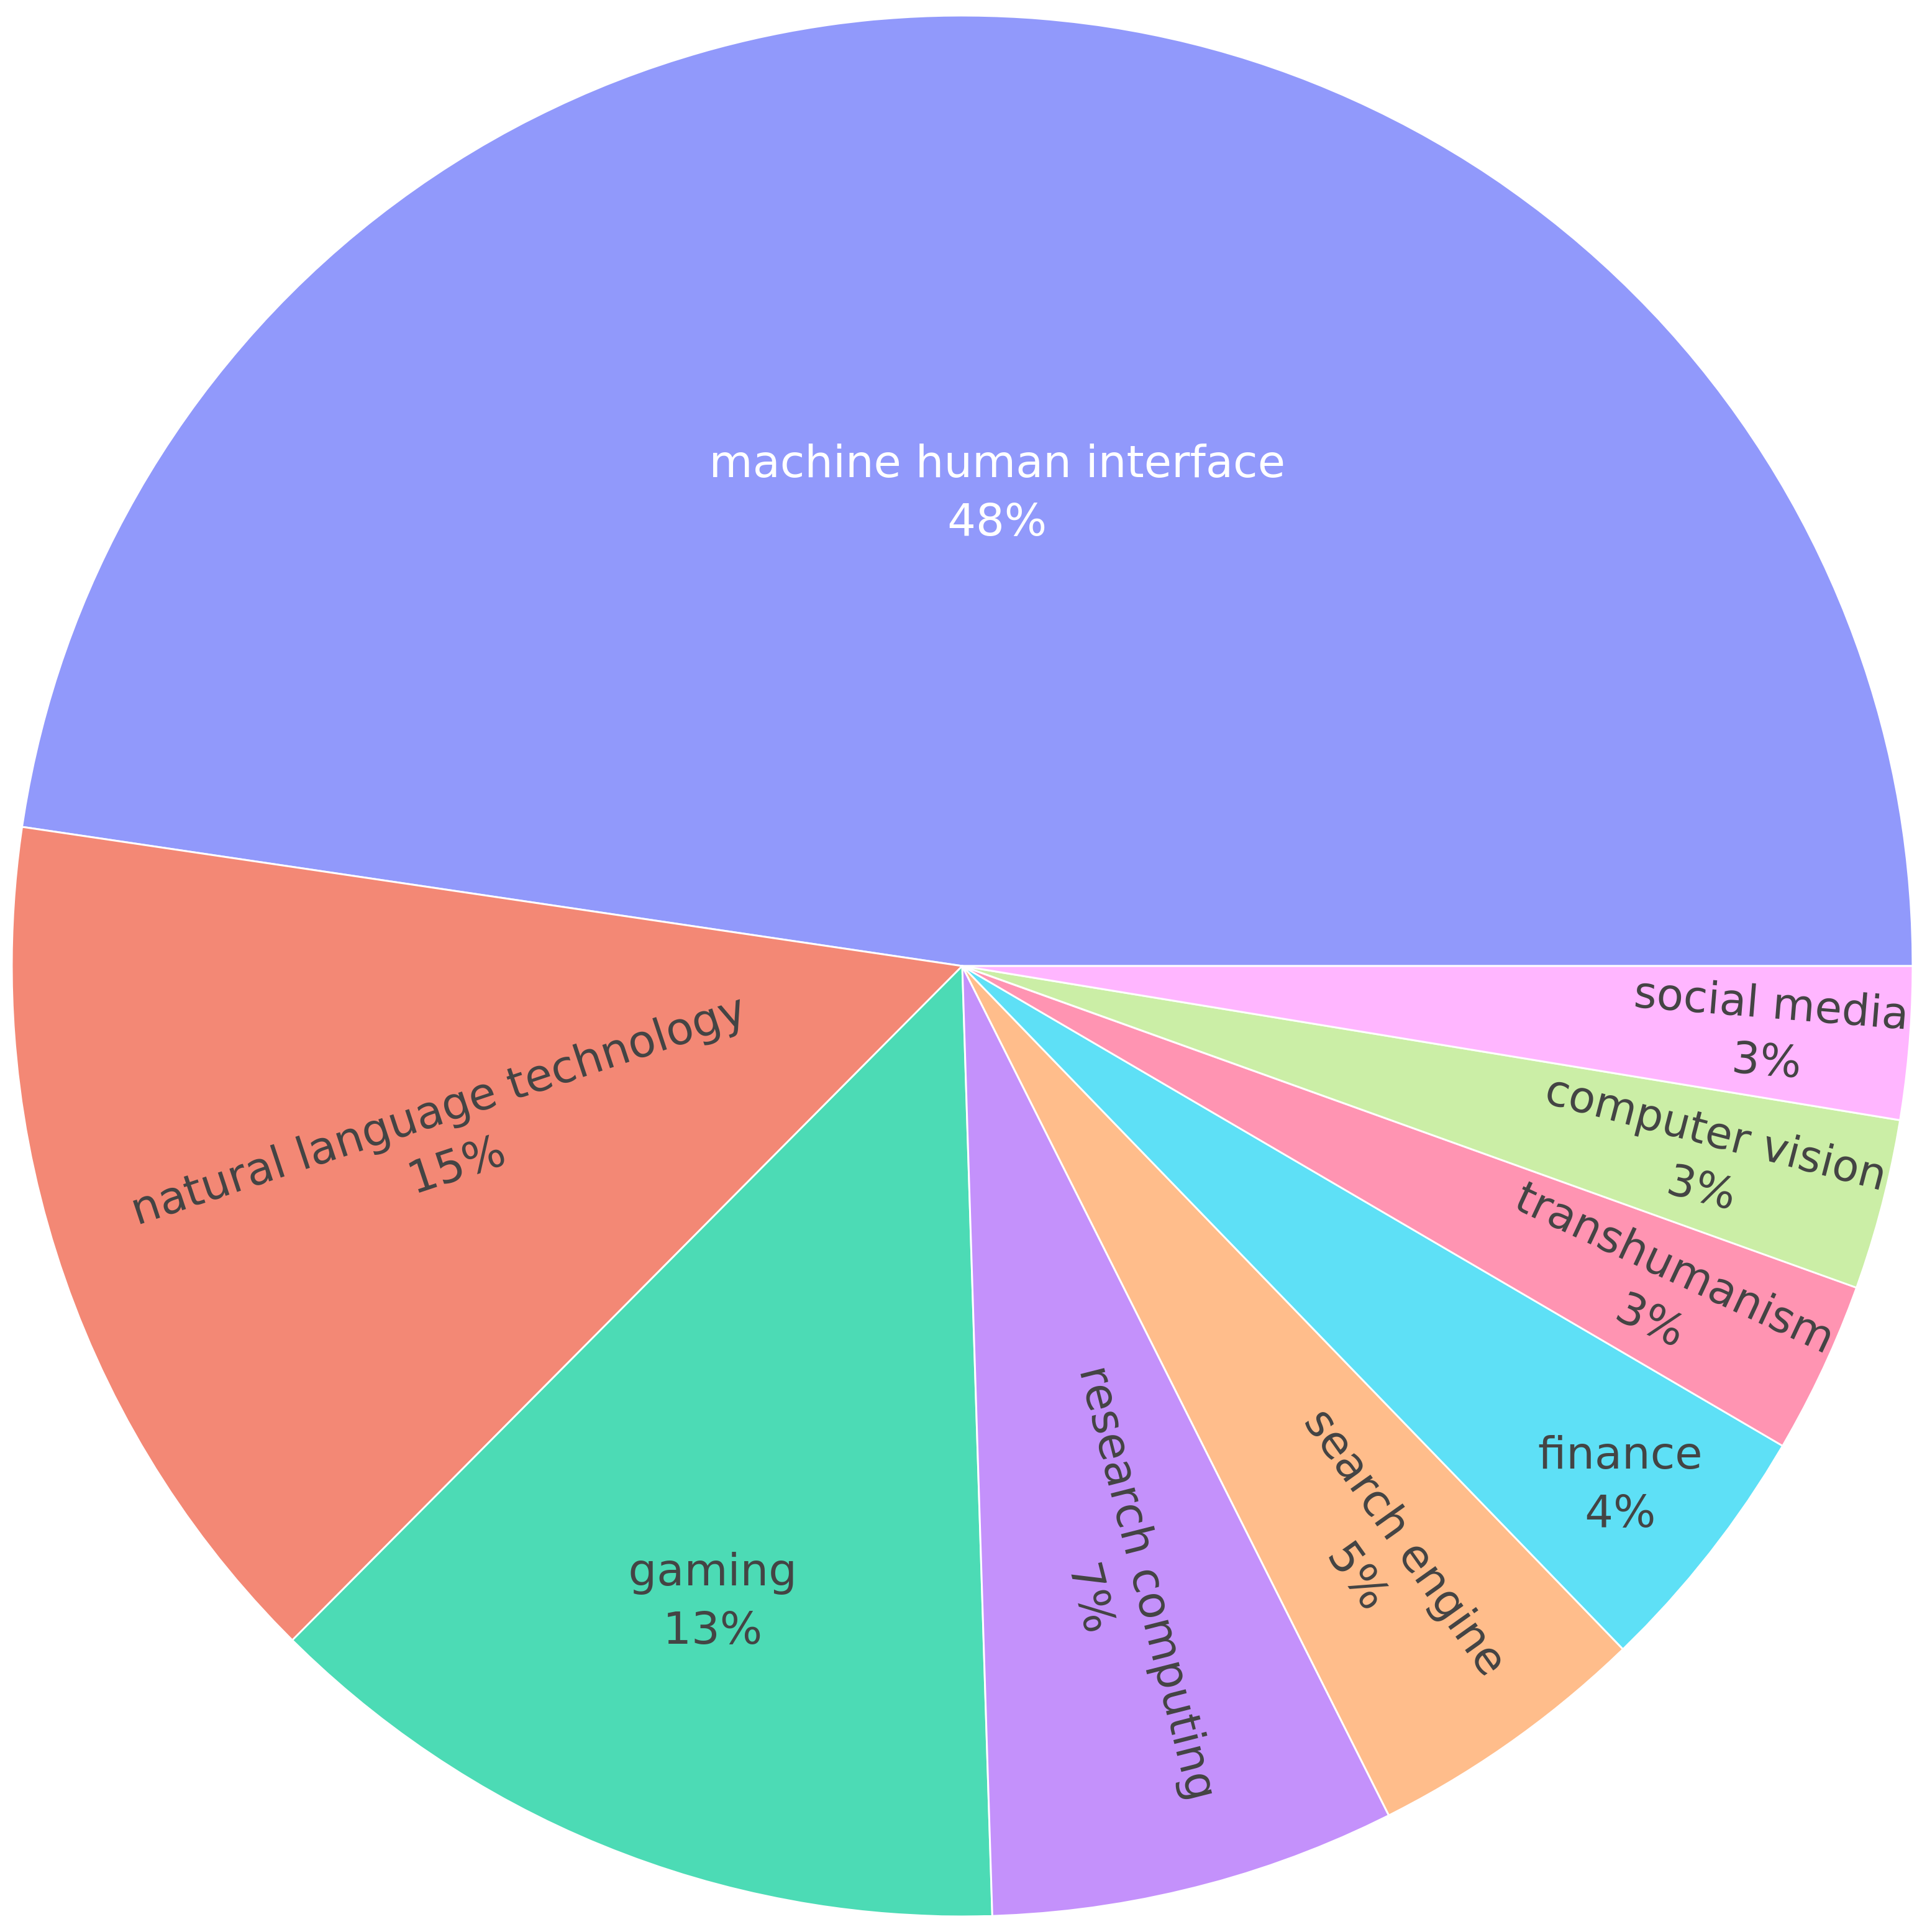
\includegraphics[width=0.6\textwidth]{pie_topics_by_occ}
    \caption{
        Dummy caption.
        Dummy caption.
        Dummy caption.
        Dummy caption.
        Dummy caption.
        Dummy caption.
        Dummy caption.
        Dummy caption.
        Dummy caption.
        Dummy caption.
        Dummy caption.
        Dummy caption.
        Dummy caption.
    }
    \label{fig:pie_topics_by_occ}
\end{figure}
\pagebreak
\begin{figure}[h!]
    \centering
    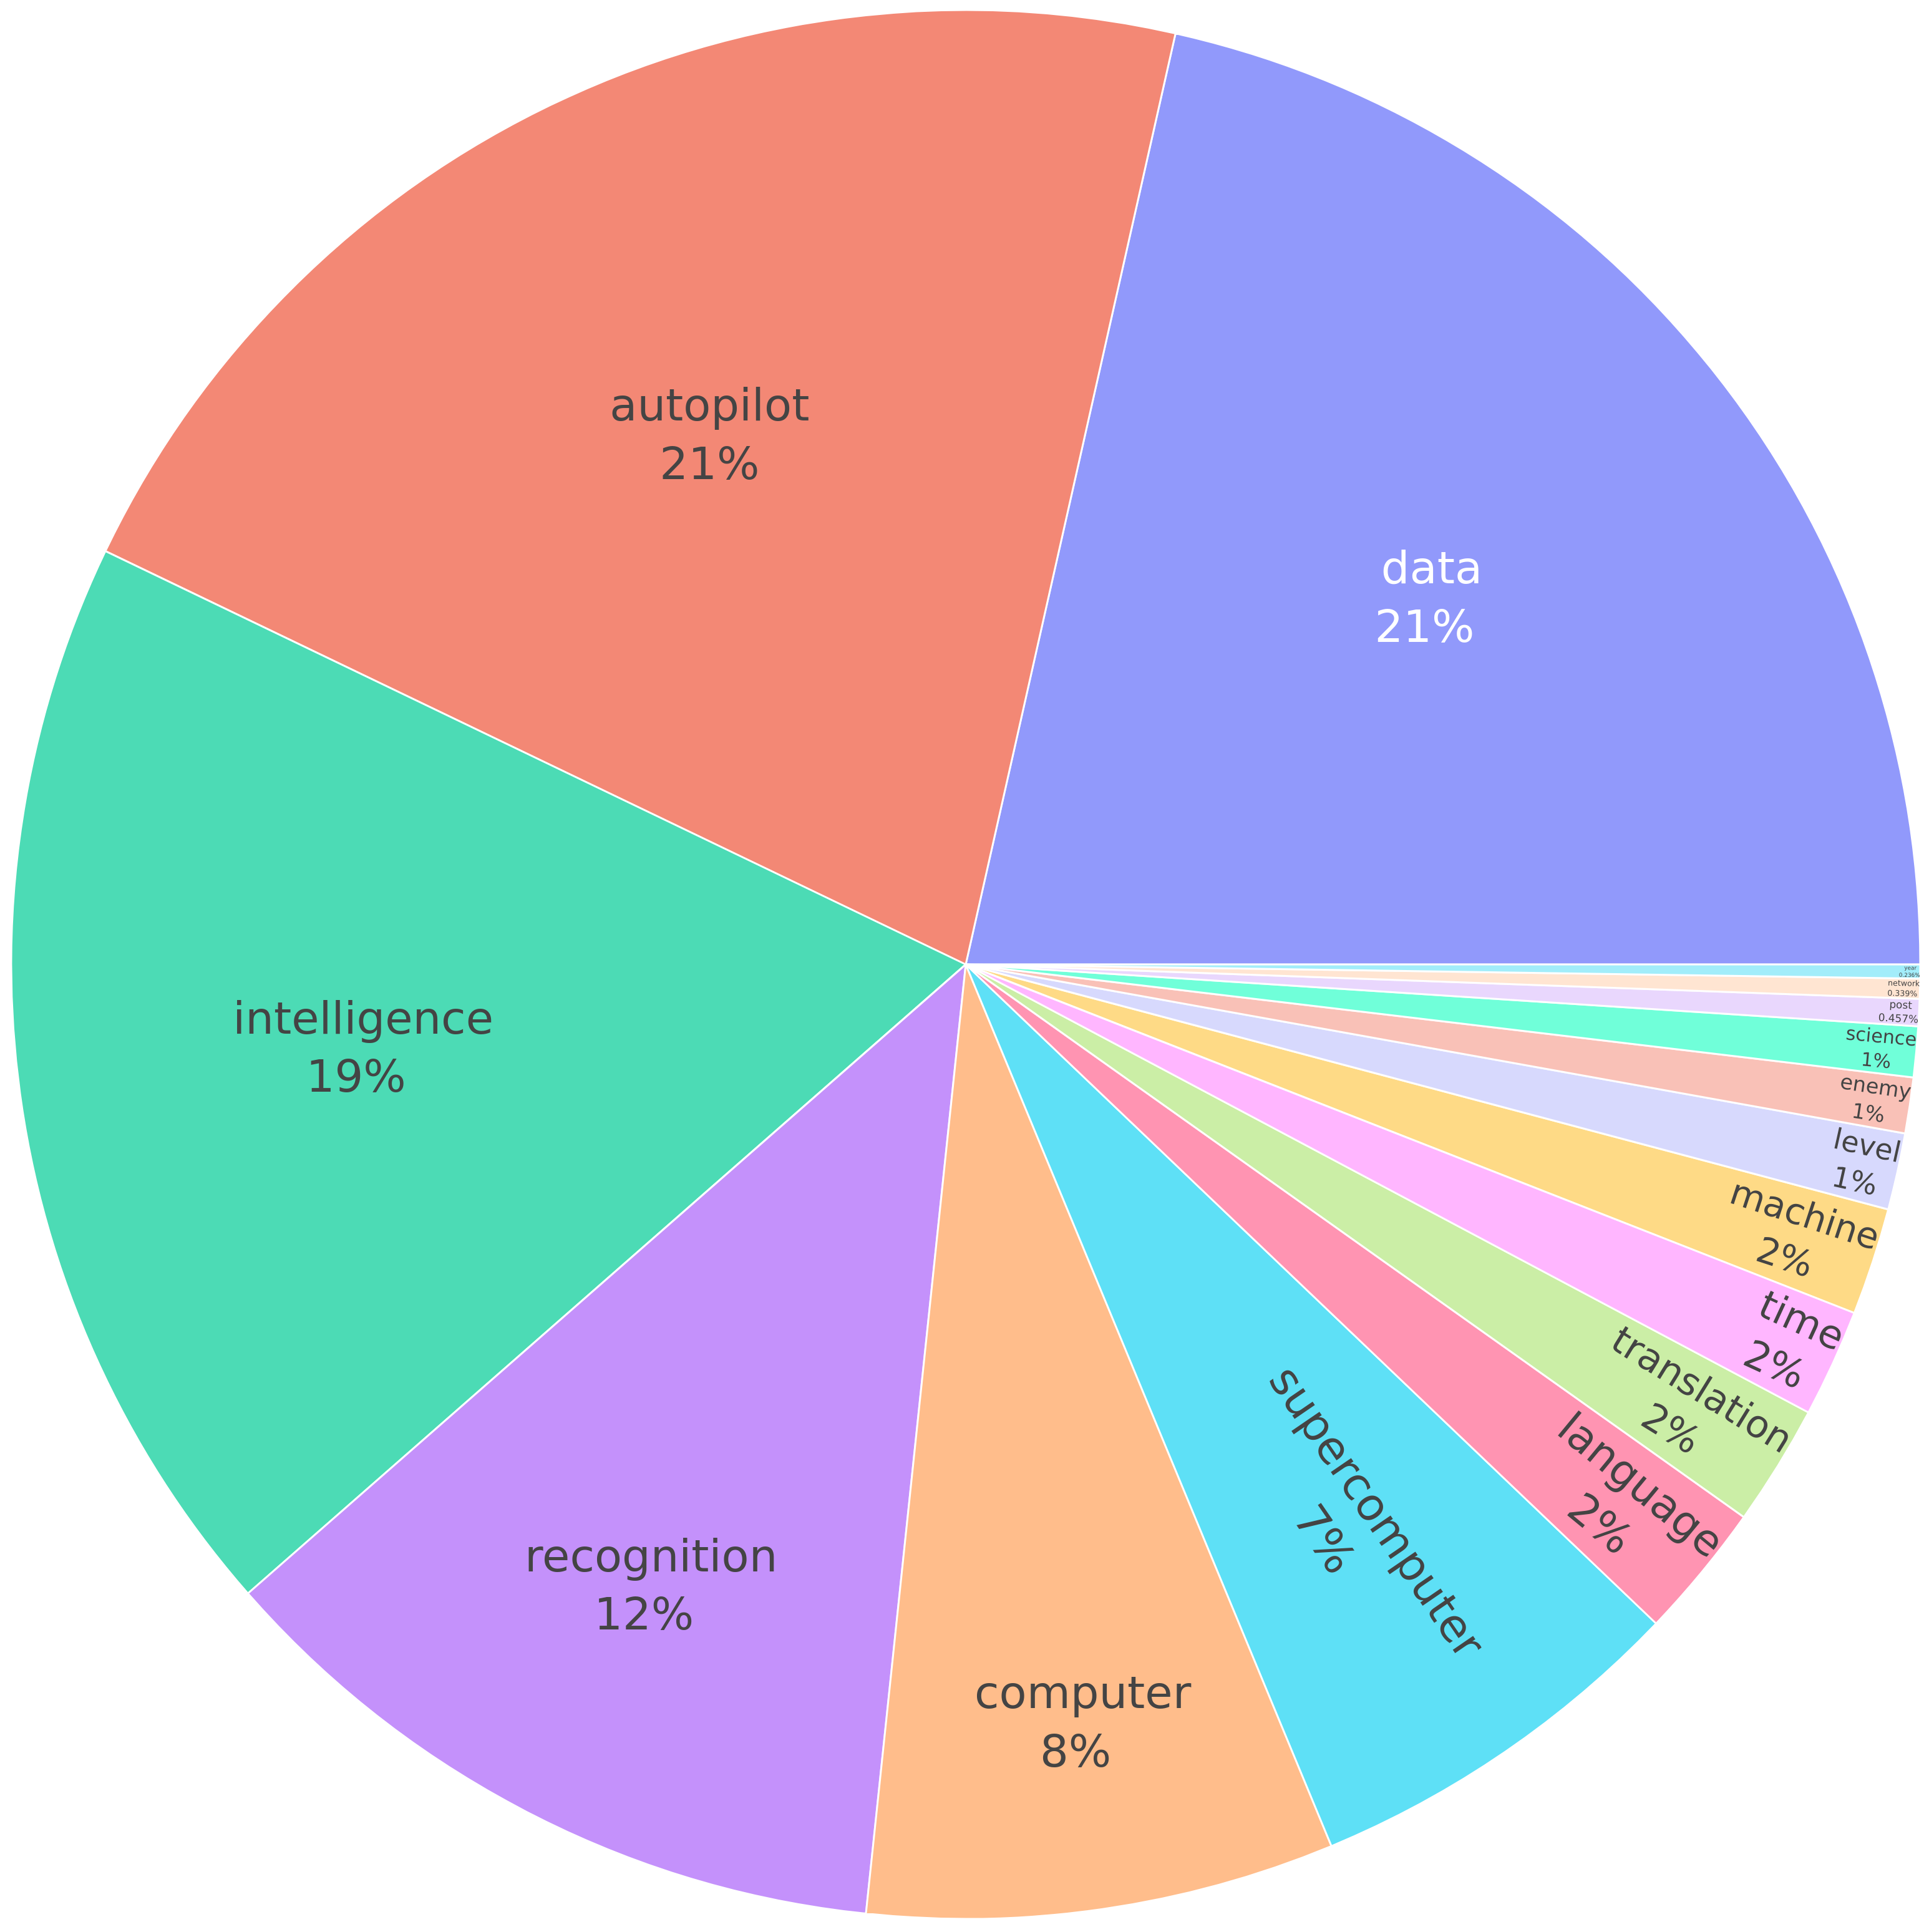
\includegraphics[width=0.6\textwidth]{pie_subtopics_by_occ}
    \caption{
        Dummy caption.
        Dummy caption.
        Dummy caption.
        Dummy caption.
        Dummy caption.
        Dummy caption.
        Dummy caption.
        Dummy caption.
        Dummy caption.
        Dummy caption.
        Dummy caption.
        Dummy caption.
        Dummy caption.
    }
    \label{fig:pie_subtopics_by_occ}
    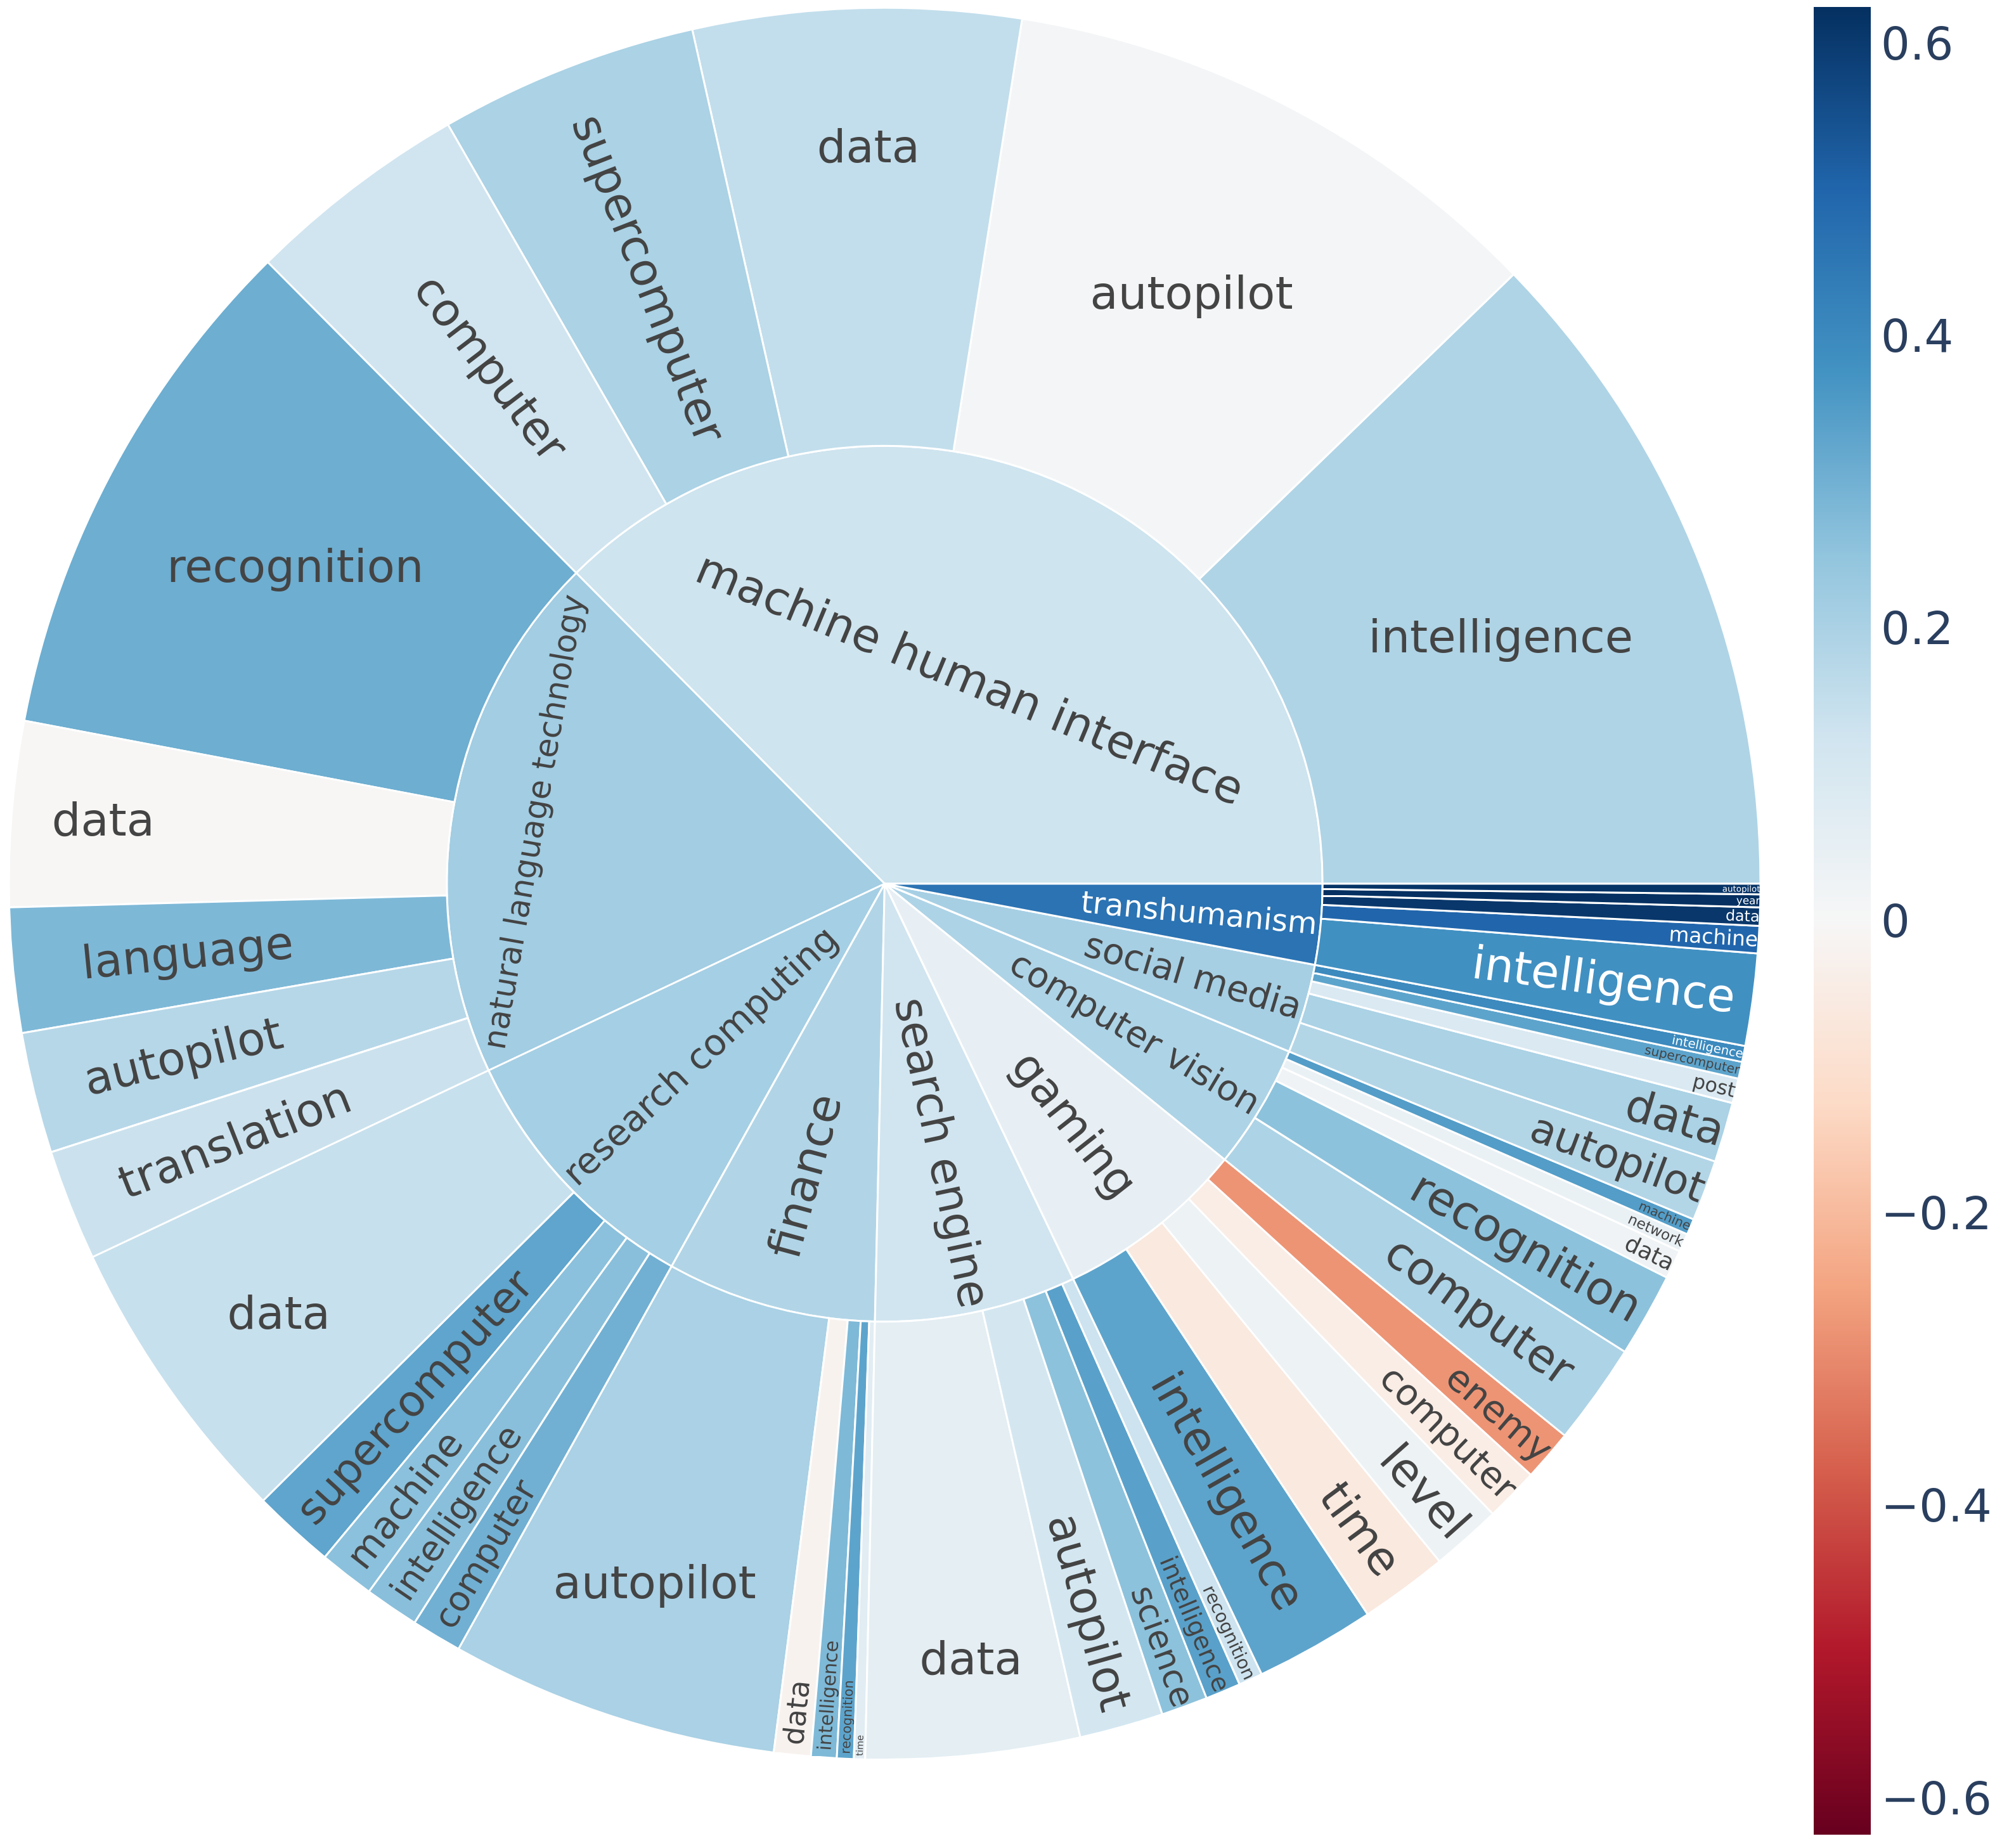
\includegraphics[width=0.6\textwidth]{pie_topics_subtopics_by_occ_sent_neu}
    \caption{
        Dummy caption.
        Dummy caption.
        Dummy caption.
        Dummy caption.
        Dummy caption.
        Dummy caption.
        Dummy caption.
        Dummy caption.
        Dummy caption.
        Dummy caption.
        Dummy caption.
        Dummy caption.
        Dummy caption.
        Dummy caption.
        Dummy caption.
        Dummy caption.
    }
    \label{fig:pie_topics_subtopics_by_occ_sent_neu}
\end{figure}


\end{document}
